\documentclass{article}
\usepackage{amsmath}
\usepackage{amsfonts}
\usepackage{multicol}
\usepackage{geometry}
\usepackage{graphicx}
\usepackage{float}
\usepackage{caption}
\usepackage{subcaption}
\geometry{legalpaper, margin=1.1in}
\title{\textbf{A Python Replication of VR-PCA Algorithm}}
\author{Ziyu  Wang}
\date{8 December 2021}

\begin{document}

\maketitle
\begin{center}
    The Oden Institute for Computational Engineering Science\\
    The University of Texas at Austin
\end{center}

\section{Abstract}
In this project, I reproduced the Variance-reduction Principal Component Analysis (VR-PCA) algorithm that was described in Shamir’s paper using Python. The code replicates the algorithms for two cases. And the project uses simulated matrices to evaluate the performance of the model based on the number of data being passed in. At the end of this project, I compared the results with the paper.

\section{Introduction}
To begin with, the principal component analysis is a frequently used feature extraction method in data analytics and machine learning problems that deal with large dimensional data sets. Given a large data set with $n$ instances (rows) and $d$ features (columns), PCA involves the idea of finding the k-dimensional subspace ($d > k$) which can project the largest variance in the data set. There are two main types for PCA algorithms, streaming and non-streaming. The article from Yang et al.[5] proposed a streaming PCA algorithm, History PCA, which is designed to solve the memory issue when dealing with large scale data. And Shamir [2][4] discussed a non-streaming algorithm called variance-reduction PCA (VR-PCA), which is the algorithm that I’ll be replicating with.\\ \\
The replication of VR-PCA algorithm is conducted under a non-streaming setting. Given a data set matrix $X\in\mathbb{R}^{d \times n}$, our goal is to find the top $k$ left singular vectors ($k\ll d$) $W$. This can be rephrased into finding the solution to the following equation, where $\| \cdot \|_F$ denotes the Frobenius norm\footnote{The Frobenius norm for a matrix $A_{m\times n}$ is defined as the square root of the sum of absolute squares of its items: $\|A\|_F=\sqrt{\sum^{m}_{i=1}\sum^{n}_{j=1} |a_{i j}|^2}$},
\begin{equation} \label{first} 
\underset{W \in \mathbb{R}^{d \times k}:W^\top W=I}{\max} \frac{1}{n}\|X^\top W\|_F^2 \end{equation}  
\\ 
Based on Shamir’s articles [2], this problem setting is equivalent to finding the top $k$ eigenvector(s) of the covariance matrix $A=\frac{1}{n}XX^\top$. The first case of this project corresponds to finding only the top eigenvector, i.e., $k = 1$, and the second case is a generalization of such. \\ \\
For $k = 1$, the VR-PCA algorithm is split into $s$ epochs, in each of which we perform a power iteration\footnote{Power iteration is used for large-scale data/matrix, when the standard eigendecomposition is not feasible. This step is shown as the calculation of $\tilde{\textbf{u}}$ or $\tilde{U}$ in the algorithms. } with respect to the covariance matrix $A$. And then we conduct $m$ stochastic updates. In each stochastic update, the algorithm uses $\textbf{x}_{i_t}$, a randomly sampled column of the matrix to “interlace with occasional exact power iterations” [4]. This step will help reduce the variance of the updates and lead to a converging result.\\ \\
For the generalized case, there are several noticeable differences in the algorithm. First, we are using an initial $d\times k$ matrix with orthonormal columns instead of the unit vector. And in the stochastic updates, we replaced the vectors by matrices and the vector normalization is replaced by a matrix orthogonalization. A new $k\times k$ orthogonal matrix is also being introduced to perform a unitary transformation for the stochastic updates. \\ \\
Both algorithms are provided below based on Shamir’s article [4]. \clearpage

\textbf{Algorithm 1} VR-PCA, $k=1$

\textbf{Parameters}: step size $\eta$, epoch length $m$

\textbf{Input}: Data matrix $X=(\textbf{x}_1, ..., \textbf{x}_n)$; Initial unit vector $\tilde{\textbf{w}}_0$

\textbf{for} $s=1,2,...$ \textbf{do}

    \quad$\tilde{\textbf{u}} = \frac{1}{n}\sum^n_{i=1} \textbf{x}_i(\textbf{x}_i^\top \tilde{\textbf{w}}_{s-1})$
  
    \quad$\textbf{w}_0 = \tilde{\textbf{w}}_{s-1}$  
  
        \quad\textbf{for} $t = 1,2,...,m$ \textbf{do}  
        
        \quad\quad\quad Pick $i_t \in \{1,...,n\}$ uniformly  
            
         \quad\quad\quad $\textbf{w}'_t = \textbf{w}_{t-1}+\eta (\textbf{x}_{i_t}(\textbf{x}^\top_{i_t}\textbf{w}_{t-1}-\textbf{x}^\top_{i_t}\tilde{\textbf{w}}_{s-1}) + \tilde{\textbf{u}})$ 

         \quad\quad\quad $\textbf{w}_t = \frac{1}{\|\textbf{w}'_t\|}\textbf{w}'_t$  

     \quad\textbf{end for}  

     \quad$\tilde{\textbf{w}_s} = \textbf{w}_m$  

\textbf{end for}\\

\textbf{Algorithm 2} VR-PCA, $k>1$

\textbf{Parameters}: Rank $k$, Step size $\eta$, epoch length $m$

\textbf{Input}: Data matrix $X=(\textbf{x}_1, ..., \textbf{x}_n)$; Initial $d\times k$ matrix $\tilde{W}_0$

\textbf{for} $s=1,2,...$ \textbf{do}

    \quad$\tilde{U} = \frac{1}{n}\sum^n_{i=1} \textbf{x}_i(\textbf{x}_i^\top \tilde{W}_{s-1})$
  
    \quad$W_0 = \tilde{W}_{s-1}$  
  
        \quad\textbf{for} $t = 1,2,...,m$ \textbf{do}  
        
        \quad\quad\quad $B_{t-1}=VU^\top$, where $USV^\top$ is an SVD decomposition of $W_{t-1}^\top \tilde{W}_{s-1}$
        
        \quad\quad\quad Pick $i_t \in \{1,...,n\}$ uniformly  
            
         \quad\quad\quad $W'_t = W_{t-1}+\eta (\textbf{x}_{i_t}(\textbf{x}^\top_{i_t}W_{t-1}-\textbf{x}^\top_{i_t}\tilde{W}_{s-1}B_{t-1}) + \tilde{U}B_{t-1})$ 

         \quad\quad\quad $W_t = W'_t(W^{'\top}_t W'_t)^{-1/2}$  

     \quad\textbf{end for}  

     \quad$\tilde{W_s} = W_m$  

\textbf{end for}

\section{Method}
First of all, to simplify and optimize the algorithm runtime, I used a simulated matrix instead of a real-world data set. Due to memory limitation, instead of constructing a $200000\times10000$ data matrix as stated in Shamir’s paper, I reduced the dimension into a $500\times100$ matrix for $k=1$ case and a $250\times50$ matrix for $k>1$ cases. The other parameters maintain the same logic as Shamir’s discussion [2]. The epoch length $m$ is set to be equal to the number of instances (rows) $n$, and the step size $\eta$ is set to be $\eta=\frac{1}{\bar{r}\sqrt{n}}$, where $\bar{r}=\frac{1}{n}\sum^n_{i=1}\|\textbf{x}_i\|^2$. \\ \\
There are several parameters that need to be covered in the discussion. In Shamir’s experiment, there is an assumption of eigengap $\lambda$\footnote{Shamir also discussed the different scenarios of the convergence rate with and without an eigengap assumption. Such discussion can be found in another paper [3].}, which is the difference between two successive eigenvalues. We use this assumption in the creation of matrices. In this replication, there are 5 different eigengap choices, stored in an array. To use these eigengaps in creating the matrix, we first need to construct a $d\times d$ diagonal matrix $D$ with diagonals ($1,1-\lambda,1-1.1\lambda,…,1-1.4\lambda,q_1,q_2$,…), where $q_i=\frac{|g_i|}{d}$ and each $g_i$ is chosen according to a standard Gaussian distribution. Then we create two random orthogonal matrices $U_{d\times d}$ and $V_{n\times d}$ to form data matrix $X$, where $X=UDV^\top$.\\ \\ 
Based on the matrix $X$, the python function then is designed to extract the first (top left) eigenvector by simply selecting the first column of $U$, as shown in Figure 1. By adding a random noise vector and normalize it, we get the initial unit vector $\tilde{\textbf{w}_0}$ that can be passed into the VR-PCA algorithm. \\ \\
The replication of the algorithm takes all the parameters specified in the pseudocode and runs with a fixed number of loops. As shown in Figure 2, at the end of each loop, I calculated the log error to measure the performance of this algorithm. The error is calculated by the following equation from Shamir’s paper [2], where $\textbf{w}$ is the vector we have obtained so far,
\begin{equation}
    log_{10}(1-\frac{\|X^\top\textbf{w}\|^2}{\underset{\textbf{v}:\|\textbf{v}=1\|}{\max}\|X^\top \textbf{v}\|^2})
\end{equation}
\clearpage
\begin{figure}[H]
    \centering
    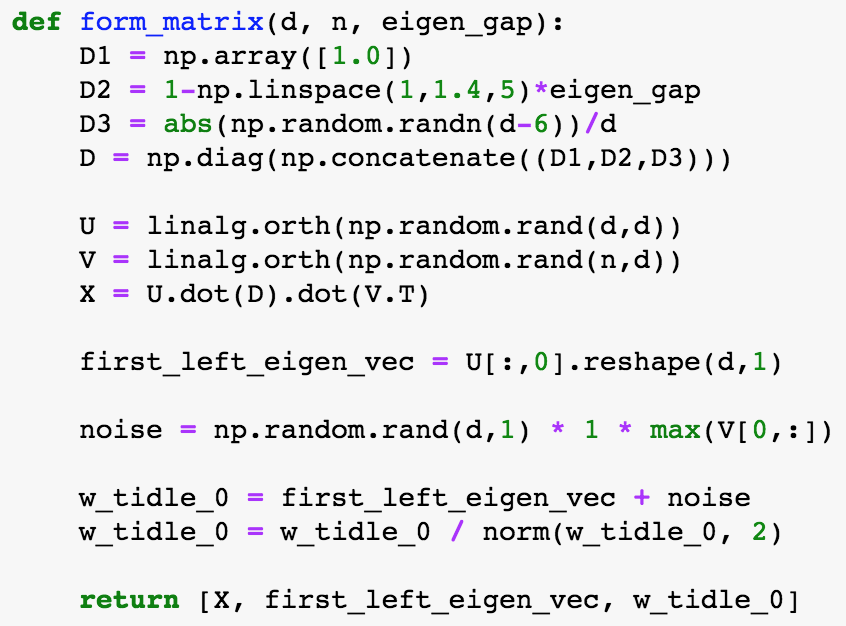
\includegraphics[scale=0.5]{./form_matrix1.png}
    \caption{Matrix formation, k=1}
\end{figure}
\begin{figure}[H]
    \centering
    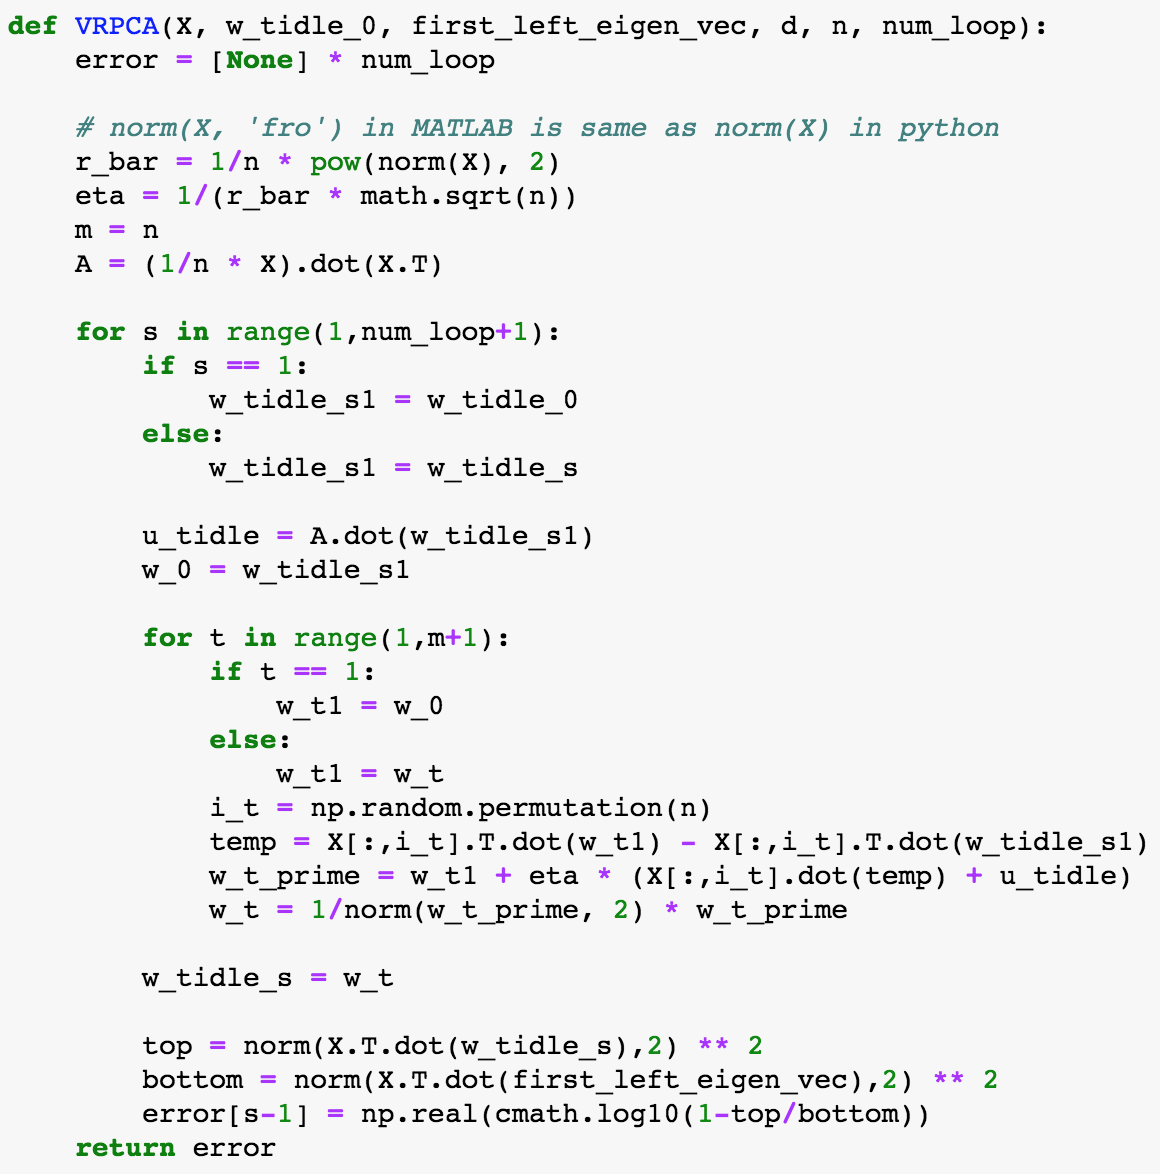
\includegraphics[scale=0.45]{./VRPCA1.png}
    \caption{VR-PCA, k = 1}
\end{figure}
With this algorithm, I then ran the experiment with several different eigengap values with the number of loops being 60. The following plot shows the result where x-axis measures the number of loops and the y-axis measures the log error calculated from the Eq. (2).
\begin{figure}[H]
    \centering
    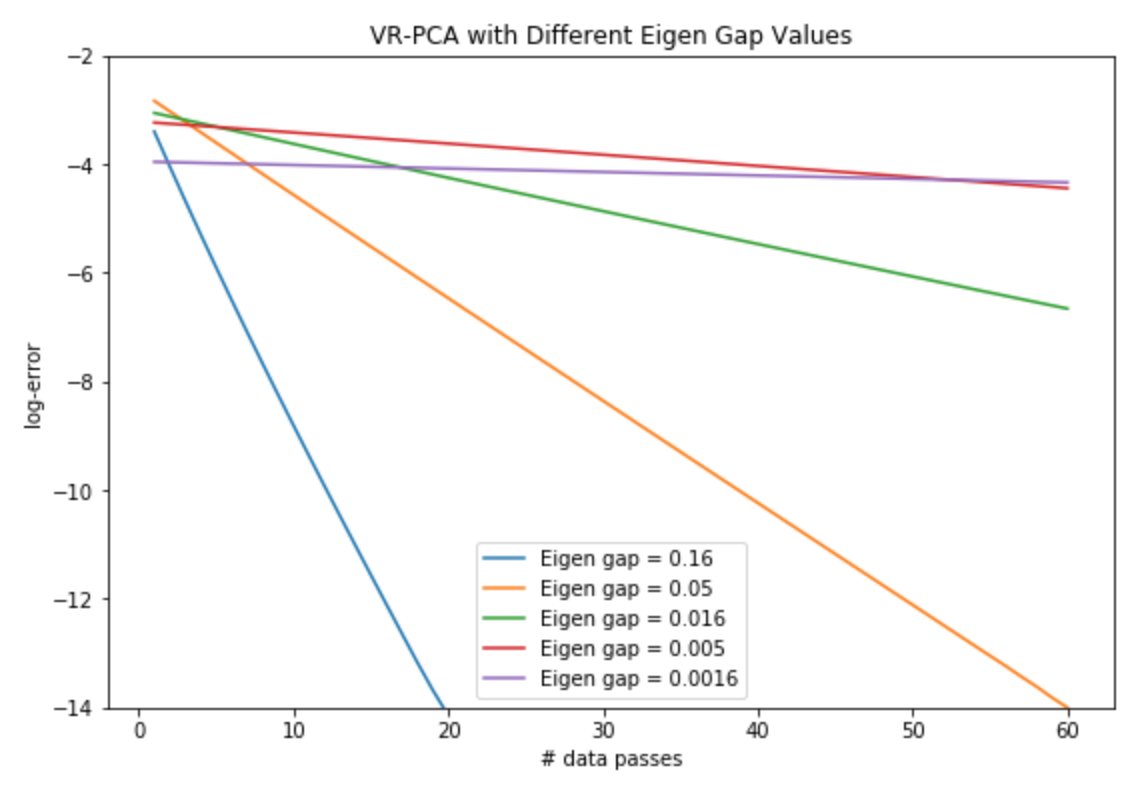
\includegraphics[scale=0.5]{./plot1.png}
\end{figure}
This plot shows that as more data being passed in and updating the algorithm, the log error is monotonically decreasing. And the decreasing rate varies across different eigengap values. Based on this result, the smaller $\lambda$ is, the slower the error decreases, and the slower the algorithm converges. It is noticeable that since the scale of error is in logarithmic, the convergence rate is in fact exponential for $\lambda$ = 0.16, 0.05, and 0.016 but sub-exponential for the other two. \\ \\
Now we move on to the replication of VR-PCA algorithm under $k>1$ cases. The matrix formation function would be very similar with a few nuances. As shown in Figure 3, instead of getting the first eigenvector, we need a $d\times k$ matrix of all top $k$ eigenvectors as the initial matrix. We use a similar approach as the previous algorithm by extracting the first $k$ columns of $U$ because the columns of $U$ are the eigenvectors corresponding to each eigenvalue of $X$ in descending order. Another change is that instead of normalization, we orthonormalized the new $d\times k$ matrix $\tilde{W}_0$ to ensure that its columns are orthogonal to each other. The orthonormalization function is provided below as well\footnote{The orthonormalization algorithm is based on Gram-Schmidt process [1].}. 
\begin{figure}[H]
    \centering
    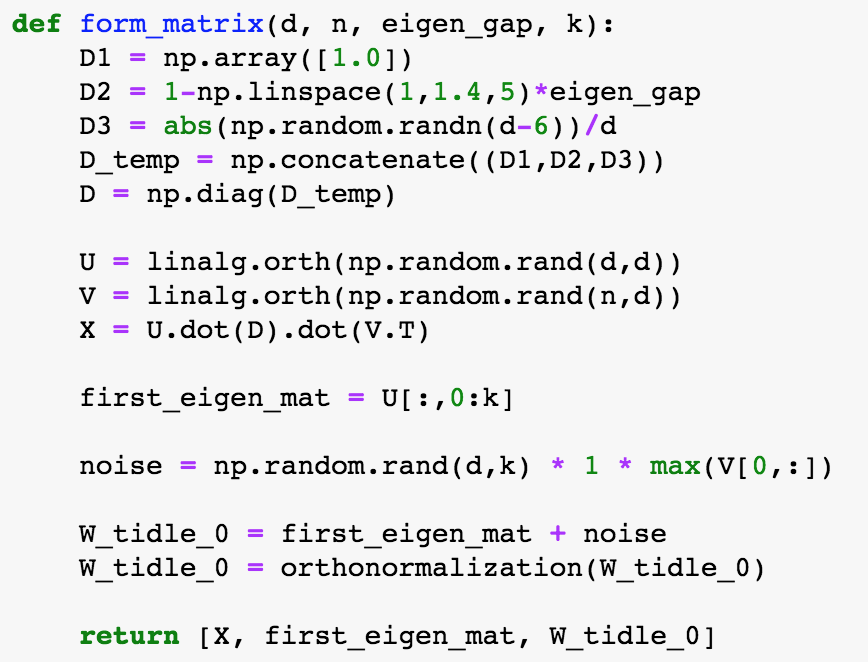
\includegraphics[scale=0.5]{./form_matrix2.png}
    \caption{Matrix formation, $k>1$}
\end{figure}
\begin{figure}[H]
    \centering
    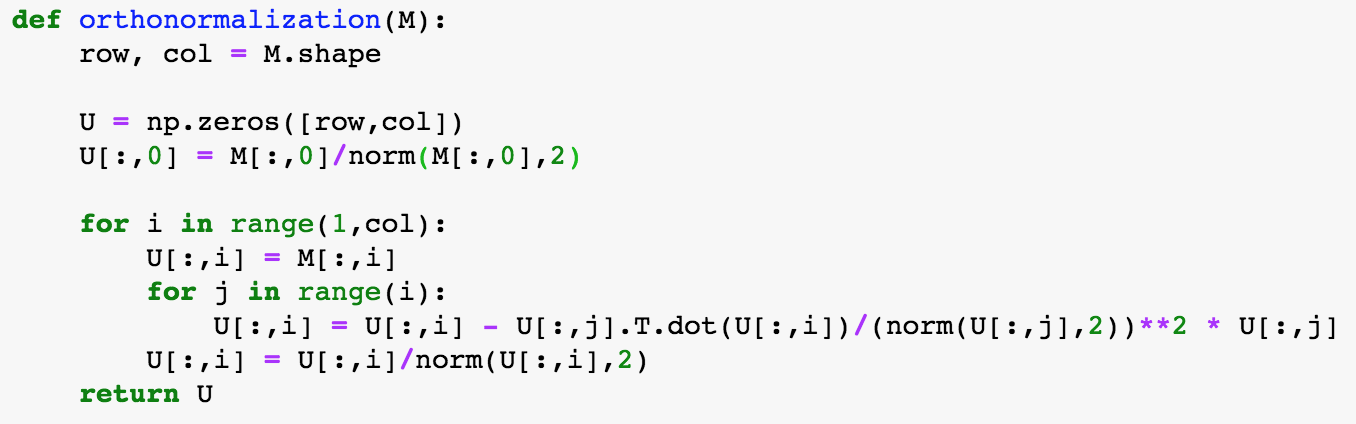
\includegraphics[scale=0.5]{./orthonormalization.png}
    \caption{Orthonormalization}
\end{figure}
After forming all necessary parameters, we can pass them into the VR-PCA algorithm for $k>1$ cases. The majority of this algorithm is similar to the previous case; but we are using a “block version”, as stated in Shamir’s paper [2]. In $k>1$ cases (Figure 6), the algorithm uses a unitary transformation in the stochastic update calculation for $\tilde{U}$ and $\tilde{W}_{s-1}$). Such transformation is done by introducing a $k\times k$ orthogonal matrix $B_{t-1}=VU^\top$, as described in the pseudocode above. Then the normalization from Algorithm 1 is replaced by an orthogonalization, finding the product of $W'_t$ and the inverse square root of $W_t^{'\top}W'_t$. The algorithm of finding the inverse square root\footnote{To find the inverse square root of a square matrix $A$, we first need to determine a matrix $V$ and a diagonal matrix $D$ such that $A=VDV^{-1}$. The diagonals of $D$ should be the eigenvalues of $A$ in descending order and $V$ is the eigenvectors. Then $A^{-1/2}=VD^{-1/2}V^{-1}$ where $D^{-1/2}$ is simply raising every diagonal entry of $D$ to the power of -1/2. } is shown in Figure 5. After each loop, we evaluate the performance of the current iteration with the following equation, 
\begin{equation}
    log_{10}(1-\frac{\|X^\top W\|^2_F}{\underset{V:\|V^\top V=I\|}{\max}\|X^\top V\|^2_F})
\end{equation}
\begin{figure}[H]
    \centering
    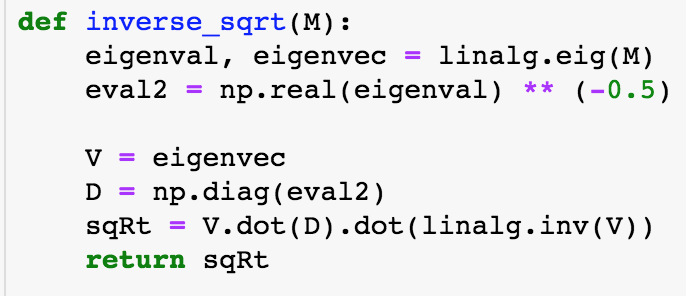
\includegraphics[scale=0.52]{./inv_sqrt.png}
    \caption{Inverse square root of a square matrix}
\end{figure}
\clearpage
\begin{figure}[H]
    \centering
    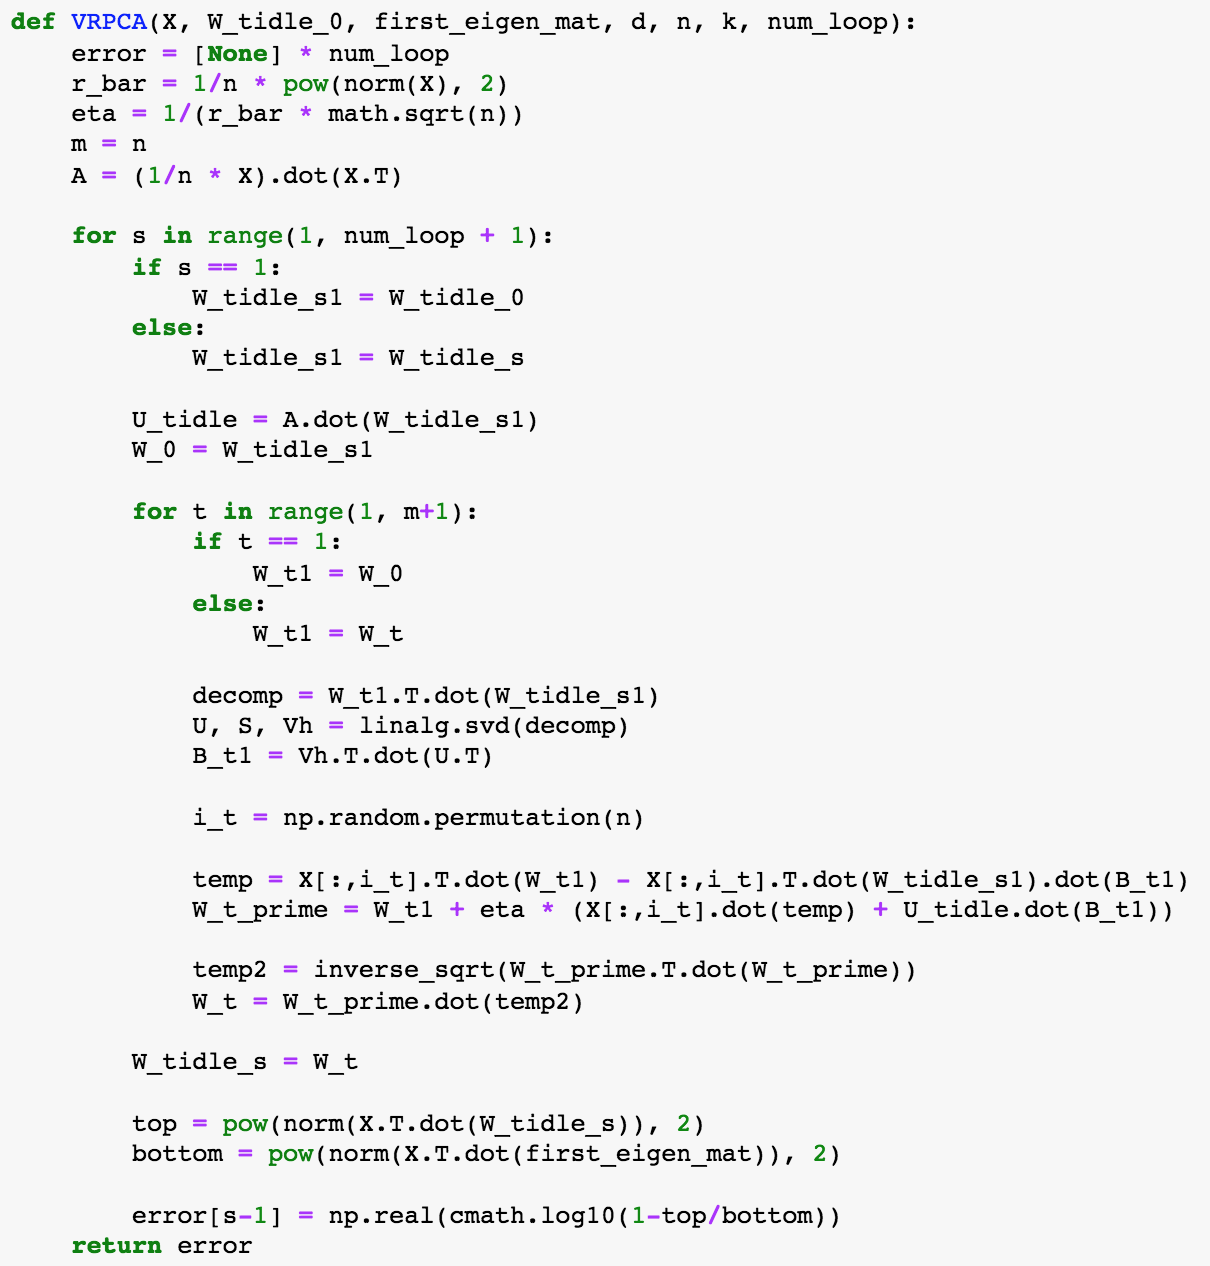
\includegraphics[scale=0.41]{./VRPCA2.png}
    \caption{VR-PCA, $k>1$}
\end{figure}
Again, similar to the $k=1$ case discussed above, we then ran this algorithm with five pre-determined eigen gap values and a fixed 60 loops. The following plots show the relationship between log errors and number of data passed in, with $k = 3$, $k = 5$, and Eq. (3). However, the results look very different from expectation as they seem to be moving up and down in a zigzag matter (Figure 7). Such result means that the algorithm does not converge but rather fluctuate around a certain value, which does not align with the theory from the paper [2][4]. It is also noticeable that when I skip the unitary transformation step\footnote{In the stochastic update step when calculating $W'_t$, the algorithm is changed into the following, \\ $W'_t = W_{t-1}+\eta (\textbf{x}_{i_t}(\textbf{x}^\top_{i_t}W_{t-1}-\textbf{x}^\top_{i_t}\tilde{W}_{s-1}) + \tilde{U})$}, the results of log error change dramatically and start to display a monotonically decreasing relationship, as shown in Figure 8. \\ \\ 
Such result is unexpected and will need further exploration. A possible reason for such result is a coding error while replicating the algorithm. The error is likely to be occurred in either the creation of $B_{t-1}$ or the calculation of inverse square root of $W_t^{'\top}W'_t$. But the debugging process so far remains fruitless. 

\begin{figure}[h]
    \centering
    \begin{subfigure}[h]{\textwidth}
        \centering
        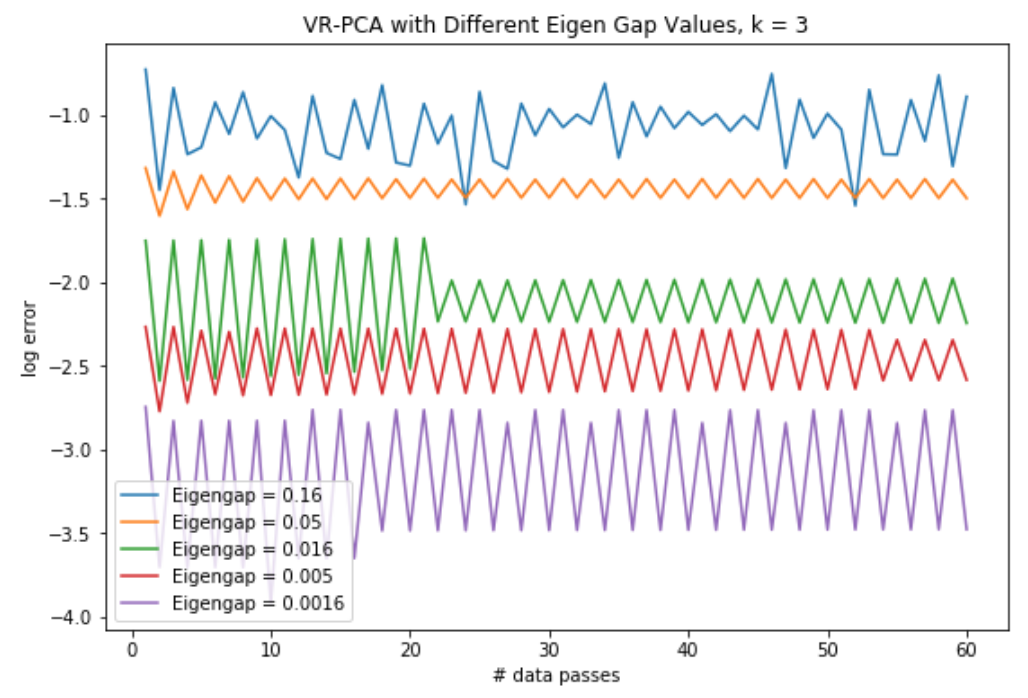
\includegraphics[scale=0.45]{./plot2_1.png}
    \end{subfigure}
    ~
    \begin{subfigure}[h]{\textwidth}
        \centering
        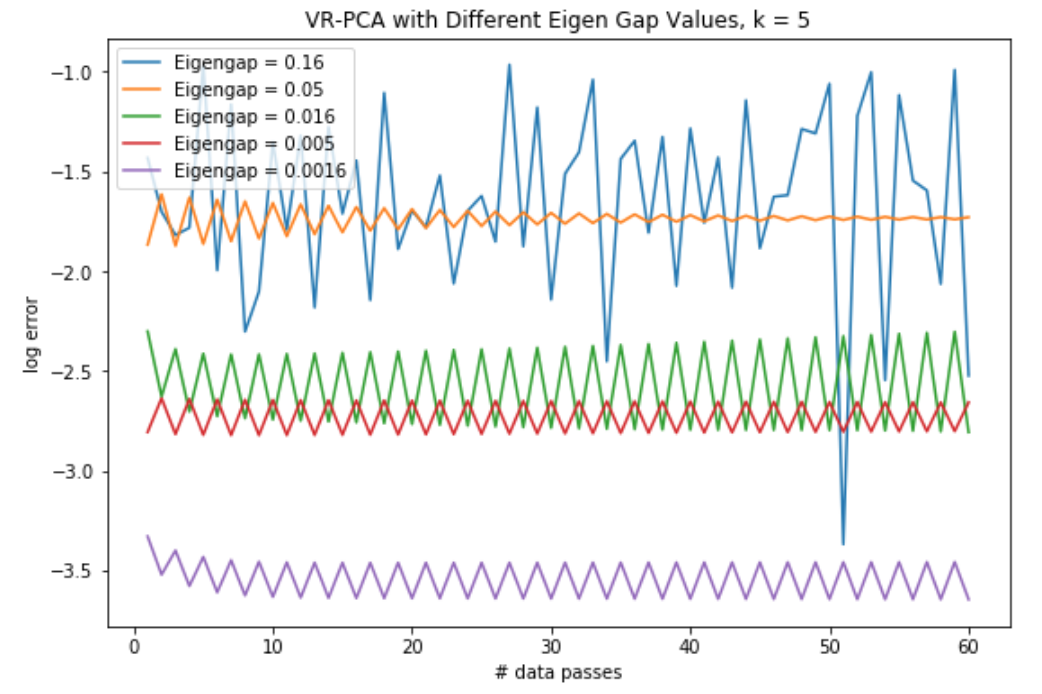
\includegraphics[scale=0.45]{./plot2_2.png}
    \end{subfigure}
    \caption{Result of VR-PCA, k = 3 and k = 5}
\end{figure}
\begin{figure}[H]
    \centering
    \begin{subfigure}[h]{\textwidth}
        \centering
        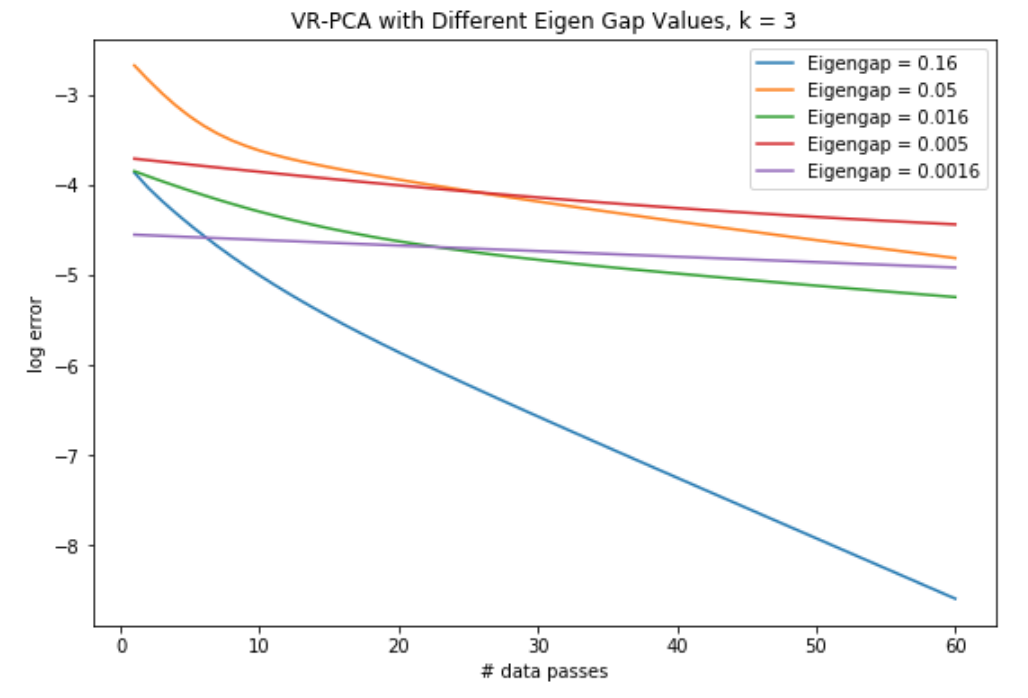
\includegraphics[scale=0.45]{./plot3_1.png}
    \end{subfigure}
    ~
    \begin{subfigure}[h]{\textwidth}
        \centering
        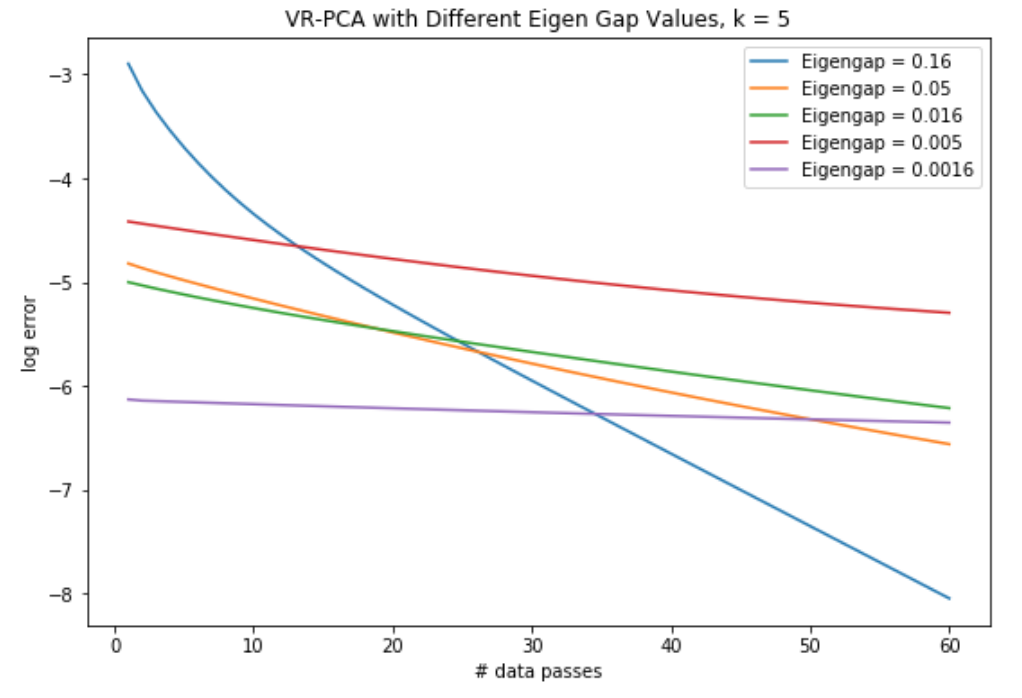
\includegraphics[scale=0.45]{./plot3_2.png}
    \end{subfigure}
    \caption{Result when excluding unitary transformation}
\end{figure}

\section{Conclusion}
In this paper, I tried to replicate a new principal component analysis algorithm, VR-PCA, that was introduced from Shamir’s papers using Python. The script uses the VR-PCA algorithms proposed by Shamir and tried to show a similar result. For $k = 1$ case, the project successfully produced a similar result using a much smaller simulated data matrix. For the $k > 1$ case, the original paper provided an example for MNIST and CCAT datasets instead of a simulated data. But the result I produced did not look like Shamir’s even qualitatively, which implies a need for debugging. And since the result changes drastically after I removed part of the code, the replicated algorithm needs further cross-check and examination. \\ \\
Overall, I personally learn and understand a lot more about principal component analysis and how it would be useful in machine learning, data visualization, and data analytics. The replication process also helped me to understand the logic and principles for this newly introduced VR-PCA algorithm. Although there are lots of professional theorems and concepts that I have not fully understood from the articles, this project gave me a productive start on how to work on an individual research project.\\ \\
\textsc{Acknowledgement}\\
This research paper is for the course \emph{CSE 370: Individual Research}, a requirement for the Computational Science and Engineering Certificate by Oden Institute at the University of Texas at Austin. I want to thank Dr. Bui for overseeing this project and Van Hai Nguyen for providing a MATLAB template to start with this project. 

\begin{thebibliography}{5}
\bibitem{wiki}
“Gram–Schmidt Process.” \emph{Wikipedia}, Wikimedia Foundation, 8 Sept 2021, https://en.wikipedia.org/wiki/Gram\%E2\%80\%93Schmidt\_process\#The\_Gram\%E2\%80\%93Schmidt\_process.

\bibitem{shamir1}
Shamir, O. A Stochastic PCA and SVD Algorithm with an Exponential Convergence Rate. \emph{arXiv: 1409.2848, 2015}. 

\bibitem{shamir2}
Shamir, O. Convergence of Stochastic Gradient Descent for PCA. \emph{arXiv: 1509.09002, 2016}.

\bibitem{shamir3}
Shamir, O. Fast Stochastic Algorithms for SVD and PCA: Convergence Properties and Convexity. \emph{arXiv: 1507.08788, 2015}.

\bibitem{yang}
Yang, P., Hsieh, C., Wang, J. History PCA: A New Algorithm for Streaming PCA. \emph{arXiv: 1802.05447, 2018}. 

\end{thebibliography}

\end{document}

